\section{Experiments}
\textcolor{red}{Discuss the experiments that you performed. The exact experiments will vary depending on the project, but you might compare with prior work, perform an ablation study to determine the impact of various components of your system, experiment with different hyperparameters or architectural choices. You should include graphs, tables, or other figures to illustrate your experimental results.}

=======
\textcolor{red}{discuss the experiments that you performed. The exact experiments will vary depending on the project, but you might compare with prior work, perform an ablation study to determine the impact of various components of your system, experiment with different hyperparameters or architectural choices. You should include graphs, tables, or other figures to illustrate your experimental results.}
We trained the network for about two weeks, looking for the perfect set of parameters. However, two days before delivery we found a bug that invalidated all our results. We was instantiating the training, validation and test set with the same python method with a parameter, that indicated what kind of dataset we needed. The training and validation accuracy was coherent and was going up and down as we changed the hyperparameters, but the fine tuning task was not giving good results. In addition the evaluation of the network was randomic: once it was coherent with the training and validation accuracy, another time was completely different. We debug for many days until we found that probably the computational graph wasn't build too well in case of shared methods (we had not found any literature about this). So we created three distinct (and mostly equal) functions that retrieve the training, validation and test set: this organization let us training and evaluating the network. However the time was too little to train the network sufficiently. We will report the partial training and we will show the complete results as soon as possible or at the oral presentation.\newline
The experimental part is made up of two different parts even if the fine-tuning part depends mostly on the results of the pretext task. 

% ------------------------------------------------------------------------------------------------ %

\subsection{Jigsaw puzzle task performance}
As seen in \ref{sss:PC_arch} and \ref{sss:GCP_arch} we used two different network architectures to train the Jigsaw puzzle that served two different purposes:
\begin{itemize}
    \item the PC network to implement the paper pretext task \emph{as-it-is};
    \item the GCP network to try to outperform previous results in performances and execution time.
\end{itemize}
The training tactics have been slightly different, so they will be presented in two separated sections.

\subsubsection{The PC network training}\label{sss:PC_training}
We trained the PC network making use of those assumptions:
\begin{itemize}
    \item \textbf{tunable hyperparameters}: the tunable parameters were the batch size, the learning rate, its decay rate and the momentum of SGD optimizer;
    \item \textbf{hyperparameters search}: since the GPU RAM was not so big we set the batch size as high as possible to fit the entire GPU. In this way we set it to 100 both for training and validation. As regard the learning rate, its decay rate and the momentum we tried different combination until we got a good result. We read many articles to understand the best way to tune those parameters until one \cite{SGD_momentum} gave us the theory and the \textit{rule-of-thumb}: the more the momentum, the less the learning rate;
    \item \textbf{stopping policy}: we used the early stopping policy to stop the training whenever the validation loss started to increase. In this way we let the personal computer to run the session only until it was useful and to stop as soon as possible.
\end{itemize}

The best performance that we gained so far is:
\begin{table}[!ht]
    \begin{center}
        \label{tab:PC_early_results}
        \rowcolors{2}{gray!25}{white}
        \begin{tabular}{l|l}
            \rowcolor{gray!50}
            \textbf{Type} & \textbf{Value} \\
            \hline
            Training accuracy & 0.457\\
            Training loss & 2.081\\
            Validation accuracy & 0.454\\
            Validation loss & 1.915\\
            Training time & 3h33min\\
            Learning rate & 1e-3\\
            Learning rate decay & 0.97\\
            SGD Momentum & 0\\
            \hline
        \end{tabular}
    \end{center}
    \caption{Preliminary results for PC network}
\end{table}
We can see from fig. \ref{fig:early_PC_acc} and \ref{fig:early_PC_loss} that the results are promising, althtough the network started overfitting as soon as it reached the 0.45\% accuracy on validation set.

\begin{figure}[!ht]
    \centering
    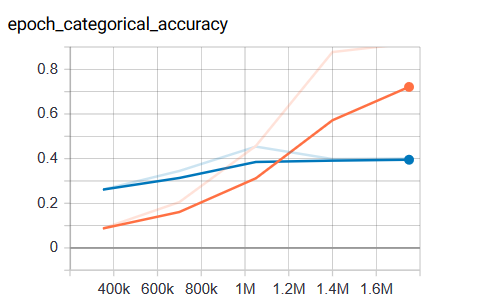
\includegraphics[scale=0.60]{images/PC_early_accuracy.png}
    \caption{Early accuracy results of PC network}
    \label{fig:early_PC_acc}
\end{figure}
\begin{figure}[!ht]
    \centering
    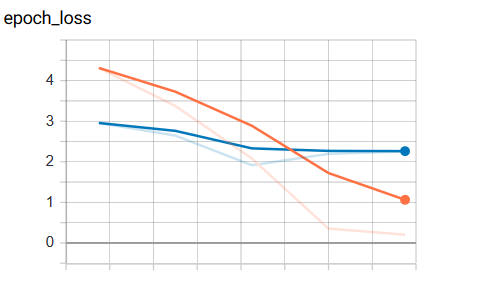
\includegraphics[scale=0.60]{images/PC_early_loss.png}
    \caption{Early loss results of PC network}
    \label{fig:early_PC_loss}
\end{figure}


\subsubsection{The GCP network training}\label{sss:GCP_training}
The training of the GCP network has been more difficult since we were free to add and remove some other layers in the network. The best configuration we found before the bug was the one explained in \ref{sss:GCP_arch} and gave very good results. However we could not trust those results and we started the training from scratch. We found that the Adam optimizer was more difficult to train since its trend is more sensible to the learning rate and tend to overfit easily. Why controlled that overfit with many batch normalization layers, that stabilized the weights between convolutions and before the output layers. With this in mind, we used those assumption to train the network:
\begin{itemize}
    \item \textbf{tunable hyperparameters}: the tunable parameters were the batch size, the learning rate, its decay rate and the momentum of the batch normalization;
    \item \textbf{position of batch norm layers}: we tried different combination to see in which position the batch normalization layers were more effective in stabilizing the training. We have seen so far that they help more before the max pool layers of the AlexNet block and before the last dropout, near the output;
    \item \textbf{hyperparameters search}: to stabilize the training we set the batch size to 512, as high as we could. As regard the learning rate, we use it to slow down learning as much as possible, since the Adam optimizer had the tendency to converge rapidly (and to overfit). We used the learning rate decay with the same purpose. The batch normalization momentum was the trickiest hyperparameter to tune: too high parameters carried no learning, too low overfit. We took inspiration from various online articles (see for example \cite{batch_norm_online}), however none of them helped us very much. We finally found that \emph{very} high momentum values were helping us to learn without overfit. In addition we added a L2 regularization for weights and bias of the last AlexNet dense layer: this helped us to slow down learning and stabilize the loss function \cite{l2_neural_networks}. This is why the loss values are higher than the PC counterpart;
    \item \textbf{stopping policy}: as the online virtual instance of the machine is paid per hour and not per use we only set a maximum value of epochs. In case of overfitting we stopped the training as soon as we saw it.
\end{itemize}
The best performance that we gained so far is:
\begin{table}[!ht]
    \begin{center}
        \label{tab:GCP_early_results}
        \rowcolors{2}{gray!25}{white}
        \begin{tabular}{l|l}
            \rowcolor{gray!50}
            \textbf{Type} & \textbf{Value} \\
            \hline
            Training accuracy & 0.398\\
            Training loss & 4.898\\
            Validation accuracy & 0.367\\
            Validation loss & 5.202\\
            Training time & 6h6min\\
            Learning rate & 5e-6\\
            Learning rate decay & 0.80\\
            BN Momentum & 0.99 AlexNet, 0.997 last\\
            \hline
        \end{tabular}
    \end{center}
    \caption{Preliminary results for GCP network}
\end{table}
We can see from fig. \ref{fig:early_GCP_acc} and \ref{fig:early_GCP_loss} that the results are promising, althtough the network started overfitting as soon as it reached the 0.36\% accuracy on validation set.

\begin{figure}[!ht]
    \centering
    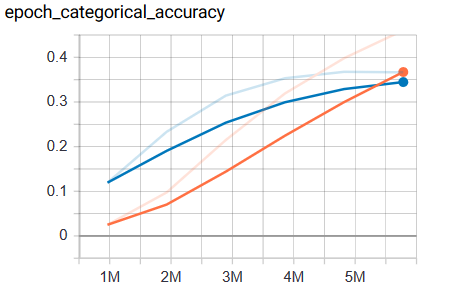
\includegraphics[scale=0.60]{images/GCP_early_accuracy.png}
    \caption{Early accuracy results of GCP network}
    \label{fig:early_GCP_acc}
\end{figure}
\begin{figure}[!ht]
    \centering
    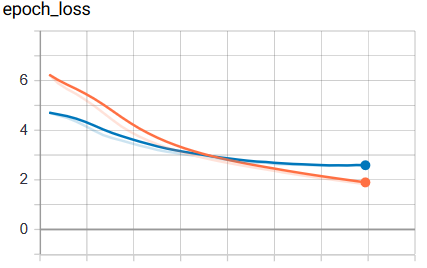
\includegraphics[scale=0.60]{images/GCP_early_loss.png}
    \caption{Early loss results of GCP network}
    \label{fig:early_GCP_loss}
\end{figure}


% ------------------------------------------------------------------------------------------------ %

\subsection{Fine-tuning on Food Dataset}
Unfortunately we could not provide any significant result for the fine-tuning task since the pretask networks were not ready to be used so far.

% ------------------------------------------------------------------------------------------------ %

\subsection{Machines details}\label{ss:machines}
The personal computer with which we have trained the pre-task neural network is a laptop with:
\begin{itemize}
    \item CPU: Intel Core i5 8300H (2.30GHz, 3.90GHz Turbo);
    \item GPU: NVidia GTX 1050 (4GB RAM);
    \item Memory: 16GB DDR4 2666MHz;
    \item Persistency: SSD Samsung 970 evo NVMe;
    \item O.S.: Windows 10 Home.
\end{itemize}
The virtual machine that we have instantiated is composed of:
\begin{itemize}
    \item vCPU: 4-core;
    \item GPU: NVidia Tesla T4 (12GB RAM);
    \item vMemory: 7.8GB
    \item Persistency: SSD 65GB;
    \item O.S.: Ubuntu 18.10.
\end{itemize}


